\documentclass[9pt]{IEEEtran}

\usepackage[english]{babel}
\usepackage{graphicx}
\usepackage{epstopdf}
\usepackage{fancyhdr}
\usepackage{amsmath}
\usepackage{amsthm}
\usepackage{amssymb}
\usepackage{url}
\usepackage{array}
\usepackage{textcomp}
\usepackage{listings}
\usepackage{hyperref}
\usepackage{xcolor}
\usepackage{colortbl}
\usepackage{float}
\usepackage{gensymb}
\usepackage{longtable}
\usepackage{supertabular}
\usepackage{multicol}

\usepackage[utf8x]{inputenc}

\usepackage[T1]{fontenc}
\usepackage{lmodern}
\input{glyphtounicode}
\pdfgentounicode=1

\graphicspath{{./figures/}}
\DeclareGraphicsExtensions{.pdf,.png,.jpg,.eps}

% correct bad hyphenation here
\hyphenation{op-tical net-works semi-conduc-tor trig-gs}

% ============================================================================================

\title{\vspace{0ex}
Model evaluation}

\author{Marko Medved\vspace{-4.0ex}}

% ============================================================================================

\begin{document}

\maketitle

\section{Cross-Validation}
Cross-validation was implemented and evaluated on four different models. 
The performance of each model was assessed using log loss and accuracy as
 evaluation metrics.
\subsection{Implementation details}
Since the dataset is assumed to be representative of the data generating process 
and the target class distribution
is imbalanced, stratified cross-validation was implemented. This ensures that eac
 fold maintains the same class distribution as the overall dataset, preventing the
  learning algorithm from encountering folds where certain classes are 
  underrepresented. By preserving class balance, the model is better equipped to 
  learn patterns from all classes and therefore the evaluation of the model is more accurate.
\\
As instructed, a baseline classifier and logistic regression were first
 evaluated. For the third model, a decision tree was chosen due to its 
 sensitivity to the minimum number of observations required to split a node —
  a key parameter that was optimized within each fold.

The parameter optimization was carried out in two ways:

\begin{itemize}
    \item \textbf{Training Fold Optimization:}  
    The model was trained on the training split of each fold, and the parameter that produced the lowest log loss on the same training data was selected.
        
    \item \textbf{Nested Cross-Validation:}  
    An additional layer of cross-validation was applied within the training split of each fold. For each parameter value, log losses from the inner folds were summed, and the parameter with the lowest total log loss was selected as the optimal value for the outer fold.
\end{itemize}

Log loss was chosen as the evaluation metric instead of accuracy because it
 is a strictly proper scoring rule — meaning it encourages the model to output
  the true class probability distribution as opposed to accuracy where only the mode of the distribution 
  is taken into account.
\\
The choice of k = 10 for cross-validation was made because decision trees are 
inherently unstable models — they are sensitive to small variations in the 
training data, which can increase variance when using a larger k. Since the
 dataset is reasonably large, 10 folds strike a good balance between bias and
  variance, providing a stable estimate of model performance without
   introducing excessive bias from smaller training sets.

A similar reasoning applies to the inner loop of the nested cross-validation. 
With only 10\% less data available in the inner loop compared to 
the outer loop, using the same value of k (10) should still maintain 
 an effective balance between training size and validation 
stability.

\subsection{Results}
In Table~\ref{tab:results}, we can observe the performance of the four models. 
Note that the uncertainty was quantified using bootstrap with 500 repetitions.

Focusing on log loss, the decision tree shows a particularly high value,
 especially when using training fold optimization. This can be attributed
  to the fact that this model is often overly confident in its predictions, 
  meaning the predicted class tends to have a very high probability.
   Consequently, in the case of misclassification, this high confidence
    leads to a larger penalty, resulting in high log loss.
     This effect is especially evident when using training fold 
     optimization, where the tree overfits more severely than in the
      nested CV case. Note that the smallest possible minimal number
       of observations required to split a node during parameter tuning
        was set to 10, which helps prevent the tree from completely 
        overfitting.

When examining accuracy, the results are more consistent when 
compared to logistic regression, which is expected since accuracy only
 considers the predicted class and not the full predicted distribution.



 \begin{table}[h]
    \begin{tabular}{l|l|l}
    Model                           & Log loss& Accuracy          \\
    \hline
    Baseline       & 1.161 $\pm$ 0.013    & 0.6121$\pm$  0.0069          \\
    Logistic Regression       & 0.672 $\pm$ 0.013 & 0.7329$\pm$   0.0060               \\
    Decision Tree  &  2.569 $\pm$ 0.095  & 0.7217$\pm$ 0.0063                \\
    Decision Tree (Nested CV)  &1.378 $\pm$ 0.059 & 0.7386$\pm$ 0.0060  
    \end{tabular}
    \vspace{2px}
    \caption{Comparison of log loss and accuracy of different models}
    \label{tab:results}
\end{table}


\section{Dependance of error on distance}

\subsection{Tree structure importance}

\begin{figure}[h]
    \centering
    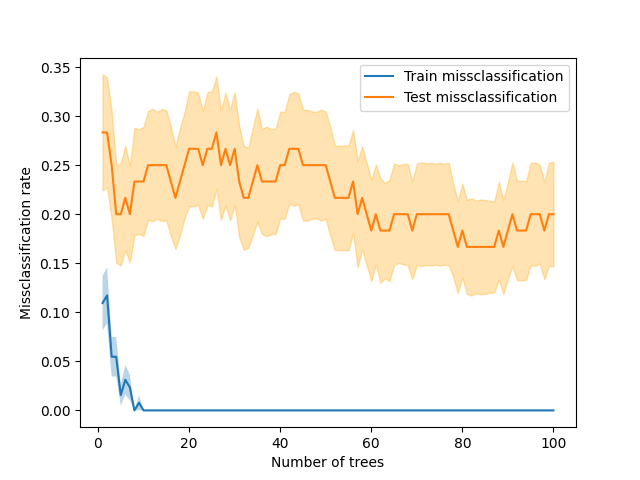
\includegraphics[width=0.95\columnwidth]{figures/missclass_num_trees.png}
    \caption{Misclassification versus the number of trees.}
    \label{fig:missclass_num_trees}
\end{figure}





\end{document}
